
This chapter provides an overview of the project in \autoref{sec:overview}, outlines the necessary modifications to the existing project to execute ExpoSE on the execution platform in \autoref{sec:fwd-z3}, and presents the discovered system-imposed limitations in \autoref{sec:limits}. It then presents the initial idea in \autoref{sec:init-test-plain}. Some of them were contingent upon the platform on which the program was executed. In this case, an Apple MacBook Pro with an M1 Pro chip. 

\section{Overview}
\label{sec:overview}


ExpoSE functions as depicted in \autoref{fig:expose-struc} starting from a component referred to as the distributor to orchestrate the process of symbolic execution. The distributor facilitates the transmission of inputs to the executor, which, as its designation implies, executes the program under test utilizing these inputs. The execution of the program produces a trace, which is subsequently returned to the executor. From this trace, the path condition corresponding to the input is communicated to the SMT Solver. The SMT Solver solves the constraints and then transmits the resulting model back to the executor, enabling the executor to extrapolate alternative inputs. These alternative inputs are subsequently relayed to the distributor, thereby initiating the entire process again. In scenarios where multiple alternative inputs are generated, these inputs are executed concurrently.

For our case, the program under test is not just one script, but consists of both the server and the client, but also of the express model, the request model and the response model. 



\begin{figure}
  \centering
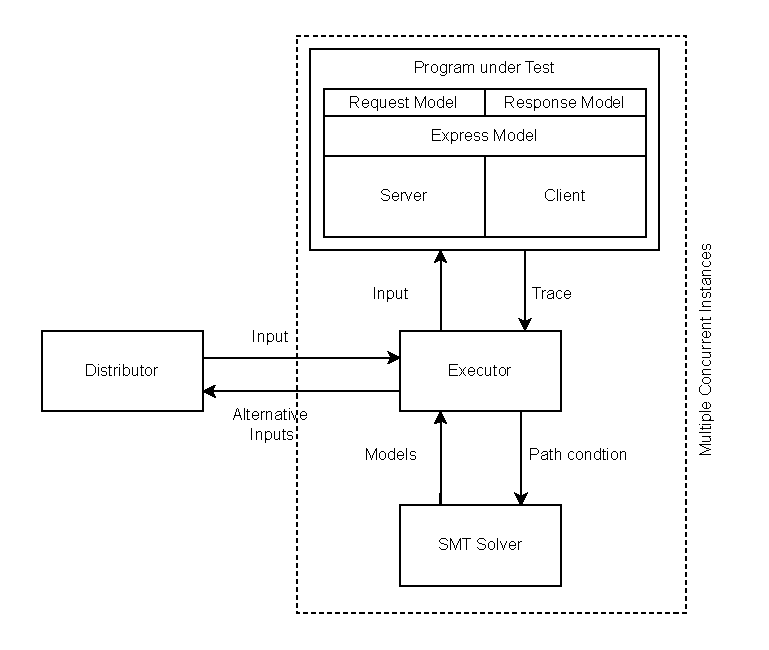
\includegraphics[width=0.7\textwidth]{exposeArchitectureDiagram.pdf}
 \caption[ExpoSE Architecture]{ExpoSE architecture structure, as depicted in \cite{loring_expose_2017}, modified to include the web application with the models for express, request, and response.}
     \label{fig:expose-struc}
\end{figure}


\FloatBarrier
\section{Forwarding Changes of Z3}
\label{sec:fwd-z3}
This section provides a short overview of the changes made to two of the four main parts that make up ExpoSE. Both were relatively simple in nature, but they were required to fix a Z3 specific internal error, that kept occurring and caused the execution to fail.

\subsection{Changes to Z3}
\label{sec:changes-z3}
As the forked repository of Z3 made for ExpoSE was almost 5 years old, and we noticed a null pointer exception in the C code, we decided to merge the changes from the original repository into the fork. We assumed that the null pointer exception had been fixed at this point because there were almost 5000 commits since the last merge. 
The forwarding went smoothly, with two exceptions. Z3 now includes the type “Char Pointer”, which had to be added to the JavaScript portion of the binding creation.

The second exception was, that the Z3 API now provides more callbacks, which required parameters that were not implemented for JavaScript. 

We deleted these callbacks, as these would stop the generation of the bindings and of the dynamically linked library (DLL) of Z3.

\subsection{Changes to Z3JavaScript}
\label{sec:changes-z3js}
With the update to Z3 itself, we also had to update the Z3JavaScript project, as this defined the types for the JavaScript bindings. It turned out to be a simple issue of adding two new object types (a {\tt{ParserContextObj}} and a {\tt{SimplifierObj}}) of the type {\tt{voidp}}, which is a pointer to the type void.


\section{System-imposed limitations}
\label{sec:limits}
In this section, we will explain the limitations imposed on the application, their consequences, and which of these consequences can or cannot be circumvented.
\subsection{JavaScript Version}
\label{sec:jsversion}
The hardest limitation of the application is that we have to stay in syntax constructs offered by the JavaScript version known as ES6 (or ECMA 2015).

This is a significant limitation, as it implies that we are unable to utilize an essential feature of contemporary JavaScript, specifically \textit{async} and \textit{await}. These two keywords refer to the asynchronous pattern that modern JavaScript employs. Without these, we will not be able to build a modern application, which is a major limitation for a server that might have to wait for resources to load or for a computation-intensive process. For these processes, we now have to rely on the practice of nesting callbacks. 




\subsection{Symbolic Addresses and Objects}
\label{sec:sym-obj}
While the other limits are specific to our use case, this issue is universal. Pointers can pose challenges for most symbolic execution engines, as highlighted in various studies, including those by~\citet{cha_unleashing_2012,coppa_rethinking_2017,elkarablieh_precise_2009}.
Reasoning about the address of a variable poses an issue, as in theory, DSE would have to assume all possible addresses. 
\citet{elkarablieh_precise_2009} propose an approach that limits every pointer to a concrete memory region in which it remains symbolically, reducing the amount of possible memory addresses, which in theory is simple, but as itself proclaims “nontrivial to implement”. 
\citet{coppa_rethinking_2017} introduce the concept of \textbf{MemSight}, which allows the mapping of symbolic expressions to data, instead of instantiated addresses, reducing the need to concretize the symbolic memory addresses. 

\citet{cha_unleashing_2012} proposed a symbolic address, which concretizes writes and only the read operations are a symbolic operation. 
A similar approach was also taken for ExpoSE, as it concretizes the namespace a variable can occupy, and only its value is resolved symbolically.
ExpoSE initializes a symbolic object by reserving a namespace, concretizing it.


On execution, it then tracks every property access, updating the initial object with a new symbolic variable for the accessed property. 
If we consider this expression:\\
\lstinline[language=JavaScript]{const object = S$.symbol("object");}
This instruction initilises the variable object as a new symbolic variable, without any indication that it is an object. 
Should ExpoSE now encounter a property access, i.e.
\lstinline[language=JavaScript]{if(object.field === "value")},
the property \lstinline[language=JavaScript]{object.field} gets initilized as a new symbolic variable
\lstinline[language=JavaScript]{object.field = S$.symbol("field");} 
and a path condition gets added, that \lstinline[language=JavaScript]{object} is, in fact, an object.\cite{loring_systematic_2021}

Although this approach works theoretically, it can cause path explosion due to JavaScript’s dynamically typed nature.
Dynamic typing in JavaScript means that variables do not have a fixed data type, and their types can change throughout program execution. This flexibility presents challenges in dynamic symbolic execution.
For instance, if a program accesses a property \lstinline[language=JavaScript]{object.foo}, the symbolic execution engine has to consider that 
\lstinline[language=JavaScript]{foo} could be a string, a number, or even an object, among others. Each of these possibilities constitutes a different path condition that the engine must track and explore. This multiplicity of paths is caused because each unique combination of types encountered at each operation increases the number of paths that must be examined. Thus, even a simple property access can lead to an explosion of paths if not handled properly, as the engine now explores additional paths for each type that the involved entity can take.

In testing engines, where the program has no other option for reasoning about the kind of inputs the program takes, using completely symbolic objects does increase coverage and helps to find bugs.
In our case, however, where we have full access to the code and where we have knowledge of all input fields, this can be avoided by creating an object with possible properties already symbolically initialized. This can be done because all unused fields are simply ignored and not adding new path conditions. 
This means, instead of waiting for ExpoSE to find \lstinline{object.field}, we start with an object already containing the field, together with a seed indicating the type  
\begin{lstlisting}[language=JavaScript]
const object = {
   "field": S$.symbol("field", "string"),
    "numberfield"; S$.symbol("numberfield", 10),
};
\end{lstlisting}

which alleviates the need of the engine to try all types possible.




\subsection{External Packages}
\label{sec:externalpack}
Our last hard limit is that ExpoSE assumes that any imported package is part of the system under test. This causes imported packages to be instrumented and execution branches to be created, which leads to a massive increase in the number of branches that have to be evaluated. While it can be used to find bugs and errors in these external packages, it does not offer any benefit for locating issues in the part of the web application we wanted to test. 
Hence, we opt out of using any external package for now.



\section{HTTP in Symbolic Execution}
\label{sec:http}
When working with web applications, there are multiple components that have to be taken care of. The internal processing, the storing and retrieving of data, and most importantly, the communication between server and client.
This communication required leads to a challenge in symbolic execution, as for it to function properly, it needs to hold the symbolic state across the many processing layers between client and server. 

The requests and responses are handled at the operating system level, converted into binaries, leaving the context to a symbolic execution engine can handle. Most symbolic execution frameworks are already limited by being language-specific. If, for example, we create a JavaScript request, we can have a symbolic state only as it exists in this context. Once it leaves the context of a JavaScript application, we would require an engine that supports multiple languages and can also operate on a system level. On the receiving end, the engine has to reverse this process, and continue with the incoming symbolic request.


There have been efforts to support this cross-language and cross-platform dynamic symbolic execution. \citet{bucur_prototyping_2014-1} introduced \textbf{Chef}, a symbolic execution framework specifically designed to address the challenges of analysing programs written in interpreted languages, such as Python or Lua. Rather than implementing symbolic semantics for each language independently, Chef takes a novel approach by transforming the interpreter itself into a symbolic executor. 
This is achieved by embedding symbolic values natively into the interpreter’s execution model, treating them equivalently to concrete values throughout program evaluation. This strategy eliminates the need to reimplement complex language semantics and runtime behaviour, which are typically tightly coupled with the interpreter's implementation.
Built on top of \textbf{S\textsuperscript{2}E}\cite{chipounov_s2e_2011}, a system-level symbolic execution platform that extends \textbf{QEMU} \cite{bellard_qemu_2005} and enables symbolic analysis of full virtual machines, including the operating system kernel, user-space programs, and network stacks. By leveraging S\textsuperscript{2}E, Chef can symbolically execute the interpreter as a binary within the VM, while maintaining control over symbolic memory, path conditions, and state management. This combination gives Chef the ability to analyse programs in their native environments with minimal modification, while still offering control over symbolic variables and execution paths.
This layered design is especially powerful in the context of web applications, since the interpreter can symbolically execute code that processes HTTP requests, interacts with databases, and performs complex control-flow logic, all while running within a fully symbolic operating system environment. This means Chef can, in theory, track symbolic inputs from low-level sources like socket buffers all the way through the application logic to the final response, allowing it to capture the entire symbolic communication channel between a client and server, provided the system stays within the supported language and execution model.

However, this potential comes at a cost. The combined use of Chef and S\textsuperscript{2}E introduces substantial performance and scalability challenges, especially in cross-platform or multi-language scenarios. Each component adds symbolic overhead, and the integration of multiple symbolic layers (interpreter, system, communication) can lead to an explosion of paths and long execution times. 

This leads us to the solution we use for our tests: we bypass the communication between client and server completely, by injecting the server into the client, or vice versa, depending on the server structure (more on that in \autoref{chapter:express}). With that, we have the full symbolic state of the execution, the data does not need to be transformed, and can simply be handed over to the request and response processing on server- and client-side. 
This approach effectively achieves the goal of symbolic communication, similar to what would be obtained with a cross-platform method, while reducing the associated computational overhead.


\section{Initial Testing of a Plain JavaScript Application}
\label{sec:init-test-plain}
After addressing all the fundamental issues, we began by creating a small server in plain JavaScript to explore whether it is possible to generate requests, process them, and return the correct response for the request. For example, a \texttt{GET} request with the URL \lstinline[language=JavaScript]+"/test"+ is handled by a \texttt{GET} route registered as \lstinline[language=JavaScript]{"/test"}, and not incorrectly by the \texttt{POST} route. 

\subsection{Idea}
\label{sec:idea}

The objective is to construct a plain JavaScript server by utilizing the http package's method “createServer” and subsequently eliminating all components that depend on http, thus skipping the actual server-client connection.
We have two goals for this: 
\begin{enumerate}
    \item  We create a server that has both static and variable routes, notably one route that consisted only of a regular expression, to test whether all routes could be found by the symbolic variable for the path alone.
    \item  We also implement a short test for injecting code into the response, by asserting that the client cannot send any script tag \lstinline[language=JavaScript]{<script><\script>} in the request data, while asserting that it has to be a valid email. Which in turn meant ExpoSE has to try to violate the assertion by creating inputs that contain a script tag and are no valid emails. 
\end{enumerate}
For the client-side, we create a bare-bones client that generates the symbolic request, and passes it over to the server by calling the onRequest method of the server, which gets called whenever a request is sent, bypassing HTTP. 

\subsection{Evaluation}
This small test application demonstrates that it is indeed possible to test a server with ExpoSE by fulfilling both requirements stated in \autoref{sec:idea}. Finding all the request routes within the server is straightforward, with one minor drawback: the regular expression route is not functional in a switch-case construct due to its use as a literal and not as a regular expression to match a string. 
The second objective is only moderately successful, as, despite demonstrating theoretically that the generation of a string containing a script tag works, it often exceeds the timeout limit, with a few exceptions in a test of 50 runs, where a matching string was immediately generated.

Despite this, we deem the initial test application a success, as it strongly suggests that it is possible to test a server, explore all possibly routes and locate issues in the validation, data processing and usage of this data. Hence, we move on from plain JavaScript to the usage of a framework, in our case, Express.
